% $Id: template.tex 11 2007-04-03 22:25:53Z jpeltier $

\documentclass{vgtc}
% final (conference style)
%\documentclass[review]{vgtc}                 % review
%\documentclass[widereview]{vgtc}             % wide-spaced review
%\documentclass[preprint]{vgtc}               % preprint
%\documentclass[electronic]{vgtc}             % electronic version

%% Uncomment one of the lines above depending on where your paper is
%% in the conference process. ``review'' and ``widereview'' are for review
%% submission, ``preprint'' is for pre-publication, and the final version
%% doesn't use a specific qualifier. Further, ``electronic'' includes
%% hyperreferences for more convenient online viewing.

%% Please use one of the ``review'' options in combination with the
%% assigned online id (see below) ONLY if your paper uses a double blind
%% review process. Some conferences, like IEEE Vis and InfoVis, have NOT
%% in the past.

%% Figures should be in CMYK or Grey scale format, otherwise, colour 
%% shifting may occur during the printing process.

%% These few lines make a distinction between latex and pdflatex calls and they
%% bring in essential packages for graphics and font handling.
%% Note that due to the \DeclareGraphicsExtensions{} call it is no longer necessary
%% to provide the the path and extension of a graphics file:
%% \includegraphics{diamondrule} is completely sufficient.
%%
\ifpdf%                                % if we use pdflatex
  \pdfoutput=1\relax                   % create PDFs from pdfLaTeX
  \pdfcompresslevel=9                  % PDF Compression
  \pdfoptionpdfminorversion=7          % create PDF 1.7
  \ExecuteOptions{pdftex}
  \usepackage{graphicx}                % allow us to embed graphics files
  \DeclareGraphicsExtensions{.pdf,.png,.jpg,.jpeg} % for pdflatex we expect .pdf, .png, or .jpg files
  \DeclareUnicodeCharacter{FB01}{fi}  % ADDED THIS LINE TO AVOID LIGATURE [MAURO]
\else%                                 % else we use pure latex
  \ExecuteOptions{dvips}
  \usepackage{graphicx}                % allow us to embed graphics files
  \DeclareGraphicsExtensions{.eps}     % for pure latex we expect eps files
\fi%

%% it is recomended to use ``\autoref{sec:bla}'' instead of ``Fig.~\ref{sec:bla}''
\graphicspath{{figures/}{pictures/}{images/}{./}} % where to search for the images
\usepackage{microtype}                 % use micro-typography (slightly more compact, better to read)
\PassOptionsToPackage{warn}{textcomp}  % to address font issues with \textrightarrow
\usepackage{textcomp}                  % use better special symbols
\usepackage{amsmath}                  % use matching math font
\usepackage{times}                     % we use Times as the main font
\renewcommand*\ttdefault{txtt}         % a nicer typewriter font
\usepackage{cite}                      % needed to automatically sort the references
\usepackage{tabu}                      % only used for the table example
\usepackage{booktabs}                  % only used for the table example

%% We encourage the use of mathptmx for consistent usage of times font
%% throughout the proceedings. However, if you encounter conflicts
%% with other math-related packages, you may want to disable it.


%% If you are submitting a paper to a conference for review with a double
%% blind reviewing process, please replace the value ``0'' below with your
%% OnlineID. Otherwise, you may safely leave it at ``0''.
\onlineid{0}

%% declare the category of your paper, only shown in review mode
\vgtccategory{Research}

%% allow for this line if you want the electronic option to work properly
\vgtcinsertpkg
\usepackage{subcaption}
%% In preprint mode you may define your own headline.
%\preprinttext{To appear in an IEEE VGTC sponsored conference.}

%% Paper title.

\title{DigiDrum - A Haptic-based Case Study}

%% This is how authors are specified in the conference style

%% Author and Affiliation (single author).
%%\author{Roy G. Biv\thanks{e-mail: roy.g.biv@aol.com}}
%%\affiliation{\scriptsize Allied Widgets Research}

%% Author and Affiliation (multiple authors with single affiliations).
%%\author{Roy G. Biv\thanks{e-mail: roy.g.biv@aol.com} %
%%\and Ed Grimley\thanks{e-mail:ed.grimley@aol.com} %
%%\and Martha Stewart\thanks{e-mail:martha.stewart@marthastewart.com}}
%%\affiliation{\scriptsize Martha Stewart Enterprises \\ Microsoft Research}

%% Author and Affiliation (multiple authors with multiple affiliations)
\author{Anca-Simona Horvath\thanks{e-mail: ancah@hum.aau.dk}\\ %
        \parbox{1.4in}{\scriptsize \centering Research Laboratory for Art and Technology \\ KOM, AAU Aalborg} %
\and Mauro Nascimben \thanks{e-mail: mana@create.aau.dk}\\ %
     \parbox{1.4in}{\scriptsize \centering Augmented Cognition Lab \\ CREATE, AAU CPH }%
\and Silvin Willemsen\thanks{e-mail: sil@create.aau.dk}\\ %
     \parbox{1.4in}{\scriptsize \centering Multisensory Experience Lab \\ CREATE, AAU CPH}}

%% A teaser figure can be included as follows, but is not recommended since
%% the space is now taken up by a full width abstract.
%\teaser{
%  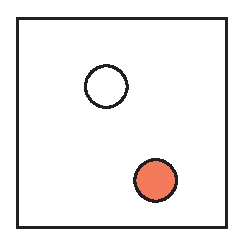
\includegraphics[width=1.5in]{sample.eps}
%  \caption{Lookit! Lookit!}
%}

%% Abstract section.
\abstract{This paper presents a novel Virtual Reality Musical Instrument (VRMI): DigiDrum, a physical drum enhanced by a vibration motor (haptuator) that provides haptic feedback using a simulated drum membrane. This same virtual membrane is sent through headphones to provide auditory feedback too. For the visual feedback, the user wears a Head Mounted Dispay (HMD) where a virtual drum aligned with the physical drum is shown and the user plays both at the same time. An experiment was performed to test whether different parameters in the membrane simulation would change the user's perception of material stiffness. Our ultimate goal is to enhance musical expression possibilities through a VRMI and to investigate whether the haptic modality influences the user's interaction. \textbf{\textleftarrow Sorry, this is pretty bad haha, please add / rewrite :)}%
} % end of abstract

%% ACM Computing Classification System (CCS). 
%% See <http://www.acm.org/about/class> for details.
%% We recommend the 2012 system <http://www.acm.org/about/class/class/2012>
%% For the 2012 system use the ``\CCScatTwelve'' which command takes four arguments.
%% The 1998 system <http://www.acm.org/about/class/class/2012> is still possible
%% For the 1998 system use the ``\CCScat'' which command takes four arguments.
%% In both cases the last two arguments (1998) or last three (2012) can be empty.

\CCScatlist{
  \CCScatTwelve{Human-centered computing}{Visu\-al\-iza\-tion}{Visu\-al\-iza\-tion techniques}{Treemaps};
  \CCScatTwelve{Human-centered computing}{Visu\-al\-iza\-tion}{Visualization design and evaluation methods}{}
}

%\CCScatlist{
  %\CCScat{H.5.2}{User Interfaces}{User Interfaces}{Graphical user interfaces (GUI)}{};
  %\CCScat{H.5.m}{Information Interfaces and Presentation}{Miscellaneous}{}{}
%}

%% Copyright space is enabled by default as required by guidelines.
%% It is disabled by the 'review' option or via the following command:
% \nocopyrightspace

%%%%%%%%%%%%%%%%%%%%%%%%%%%%%%%%%%%%%%%%%%%%%%%%%%%%%%%%%%%%%%%%
%%%%%%%%%%%%%%%%%%%%%% START OF THE PAPER %%%%%%%%%%%%%%%%%%%%%%
%%%%%%%%%%%%%%%%%%%%%%%%%%%%%%%%%%%%%%%%%%%%%%%%%%%%%%%%%%%%%%%%%

\begin{document}

%% The ``\maketitle'' command must be the first command after the
%% ``\begin{document}'' command. It prepares and prints the title block.

%% the only exception to this rule is the \firstsection command
\firstsection{Introduction}

\maketitle
Virtual Reality (VR) is described as an immersive environment experienced through sensory stimuli provided by technology. In VR, one's actions partially determine what happens in the environment \cite{Serafin:2017}. Different types of technologies are available for creating VR experiences and Head Mounted Displays (HMD) are among the most popular. VR has been used as a platform for the creation of perceptual illusions, and much research has gone into producing realistic or otherwise compelling visual and audio experiences. By comparison, the sense of touch has been neglected in spite of its obvious potential to increase a sense of presence in a simulated world \cite{Serafin:2017}.

Virtual musical instruments (VMIs) are defined as software simulations or extensions of existing musical instruments with a focus on sonic emulation. Virtual reality musical instruments (VRMIs), are those which also include a simulated visual component \cite{Serafin:2016}. In this paper we describe the design and evaluation of DigiDrum - a novel VRMI where a single physical drum is enhanced by a vibration motor (haptuator) providing haptic feedback. DigiDrum uses a physically modelled simulation of a drum membrane to map a user's tapping movements into computer generated sounds. These sounds create a vibrotactile response in the physical drum providing haptic feedback similar to what the digital sounds would produce in a real membrane. Furthermore, this sound is sent to headphones the user is wearing.  %Each physical model of a membrane is correlated to a different visual representation shown to the user in an immersive visualization through a head mounted display.

Because the drum sound is simulated, we can change its properties on the fly, something which is impossible to do in the real world. In an experiment conducted during this study, we use different combinations of values for tension of the membrane and damping (how quickly the sound dies out) to investigate which of these parameters influence the perception of material stiffness. In our test, the auditory and haptic cues are linked, or matching. A similar test has been conducted in \cite{avanzini2006}, where the influence of haptic and auditory cues on perception of material stiffness were separately tested. Furthermore, in their test, the authors used the Phantom\textregistered{} Omni\textsuperscript{TM} (now Touch) \cite{phantom} device and tested stiffness of surfaces. In this work, we try to take this research to the field of VRMIs. Another article about haptics in VMI's uses the same device \cite{passalenti2019}.

Our research question is:
\vspace{0.2cm}

\centerline{\it How can we change the user's perception of material stiffness}

\centerline{\it in an enhanced drum using auditory and haptic cues?}
\vspace{0.2cm}
\noindent Furthermore, we want to find a correlation between this perception and the way the user interacts with the drum. Our ultimate interests lie in (1) enhancing musical expression possibilities through a VRMI, and (2) investigating user's interaction with a VRMI focused not only on the visual and auditory experience, but also on haptics.
%\autoref{sec:VRMI} gives a short overview on virtual reality musical instrument state of the art.

This paper is structured as follows: \autoref{sec:Design_criteria} describes the design criteria used in the design of DigiDrum.
\autoref{sec:haptics} is an introduction to haptic perception after which \autoref{sec:myo} will give some background on the explorations done using the Myo armband \cite{myowebsite} during the course of this project. In \autoref{sec:sys} we describe the system overview. \autoref{sec:unity} details the implementation of the visual virtual environment and in \autoref{sec:PM}, the physical model sound algorithm is described. 
In \autoref{sec:exp} an experiment involving users interacting with the setup is presented with its results shown and discussed in \autoref{sec:resDisc}. Conclusive remarks and future development are discussed in \autoref{sec:conc}.

% \section{Virtual Reality Musical Instruments}\label{sec:VRMI}

\section{Design Criteria}\label{sec:Design_criteria}

We seek to create three types of illusions with our installation: a place illusion (users should feel like they are in a music production studio), a plausability illusion (users should feel like the experience is really happening) and virtual body ownership (the user should feel ownership of their virtual body, in this case - their hands). \textbf{is this all still the case?}

\section{Haptics}\label{sec:haptics}
% \subsection{Introduction}
Touch is the first sense to develop in the womb in humans \cite{Barnett1972} as opposed to vision, which is the last sense we develop. Touch is a sense which cannot be shut down whereas we can close our eyes voluntarily. Despite this, tactile awareness generally receives less attention than other sensory modalities when it comes to technological development \cite{Gallace2012}. One reason for this under-evaluation of tactile stimuli could be the broad number of sensations touch comprises: pressure, temperature, pleasure, pain, joint position, muscle sense, and movement. The experiment we are going to introduce requires subjective evaluation of drum skin vibration in form of a circular membrane. For this reason, in this section we describe in further detail haptic perception and how it works from a neurophysiological point of view as the basis for subjective decision making on tactile sensation.

\subsection{Haptic perception}
The Peripheral Nervous System gathers environmental stimuli in form of visual, audible, tactile, olfactory (smell) and gustatory (taste) inputs and transfers them to the Central Nervous System for further elaboration and integration. Tactile information is collected by proprioceptors in the skin, muscles, and joints and sent to the primary somatosensory cortex (post-central gyrus) via the dorsal column-medial lemniscus pathway to the thalamic nuclei \cite{Blatow2007}. This cortical area is the first stage for the tactile awareness occurring across body surface. The primary somatosensory cortex represents tactile stimuli following an inverted order from the toe (at the top of the parietal hemisphere) to mouth (at the lateral side of the parietal hemisphere) \cite{Narici1999}. However, several other structures of the central nervous system take part in the generation of tactile feedback, as generally, a single brain area is never responsible for the awareness of information \cite{Manzoni1986}. Directly connected with the primary somato-sensory cortex is the secondary somatosensory cortex, an associative area important in humans for light touch and tactile attention \cite{Eickhoff2005}. It is reported in literature that people undergoing tactile training improve their perception but also strengthen the connections and cortical representations of the stimulated body area \cite{Saito2007} with a direct relationship between size of cortical region and haptic performance. For the awareness of touch, the presence of the short term memory system is also important \cite{Edelman1989} as the parietal ventral area connects both pre-motor brain areas and the somatosensory memory hub. A specific area of the central parietal lobe, placed caudally from the primary somatosensory cortex, integrates the information from the visual and haptic regions to locate objects in space. 

\subsection{Technical notes on experiments involving haptics}
Conducting experiments on haptics is quite difficult because there are no proper technological devices for delivering controlled and reliable tactile stimuli \cite{Gallace2012}. In virtual environments (as used in VR) and using the Leap Motion \cite{leapwebsite} (see \autoref{sec:sys}), subjects are able to move their hands freely, which could \textbf{confound} somatosensory processing with activations related to motor planning and movement \cite{Bodegard2001}. These uncontrolled motor activities also result in uncontrolled somatic stimulation. There is an anatomical explanation of this close somato-motor functional relationship: areas involved in the perception of touch on the hands in the primary somatosensory cortex are located mostly in front of the areas responsible for hand movements \cite{Penfield1950}.
Another problem with haptics is the subjective quantification of the stimuli. Contents of tactile consciousness vary between individuals and a common lexicon to evaluate haptic sensation through surveys still seems far to be conceived \cite{Gallace2010}.

\subsection{Interaction between visual information and tactile feedback}
In famous experiment by \cite{Pavani2000}, the authors asked a group of persons to detect the position of vibrotactile stimuli while their upper arm was placed out of view and a fake rubber hand was placed in front of them. The rubber hand was placed in a position that was anatomically compatible with their real hand and all participants reported that tactile stimulation was arising from the mannequin and not from their real hand. A similar experiment was conducted by \cite{Schaefer2006} asking subjects to watch a video of a hand being touched on the first finger while their own hand was stimulated synchronously. Brain activity during synchronous stimulation showed an improved tactile acuity. Taking into account previous literature findings, we could conclude that in virtual environments hand manipulations and interactions are important factors that enhance realism and user experience. 

\section{Myo Armband}\label{sec:myo}
Myo (Thalmic Labs, now North) \cite{northwebsite} is a wireless sensor that records surface electromyographic (sEMG) activity from 8 sensors placed around the forearm. Sensors record EMG signals converting muscle activation in electric potentials. The sampling frequency of the device is 200 Hz and the signal amplitude is expressed in “units of activation” and not in millivolts (mV) like standard electromyographic recorders. The armband encloses a nine axis inertial measurement unit (IMU) which contains a three axis gyroscope, three axis accelerometer and a three axis magnetometer \cite{myowebsite}. From these measurements of spatial information, the wearer’s arm can be tracked both in the orientation and movement. The orientation data indicates the positioning of the armband in terms of the euler angles (roll, pitch and yaw). The angular velocity of the armband is provided in a vector format and the accelerometer represents the acceleration the Myo armband is undergoing at a given time. It should be considered that the Myo armband is better suited for determining the relative positioning of the arm rather than the absolute position. The Myo armband has been made to work best at the widest part of the forearm, that is, the upper forearm (\autoref{fig:arm1}).
\begin{figure}[h]
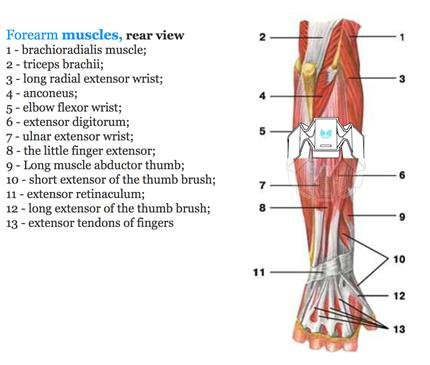
\includegraphics[width=0.5\textwidth]{myo_armband_muscles}
\caption{Muscle detected and armband position}
\centering
\label{fig:arm1}
\end{figure}
The Myo can detect the forearm movement in space, flexion and extension of the wrist and when a subject is spreading the fingers or closing the fist. 
\subsection{Raw signals and pre-processing}
To obtain gestural data from a subject after wearing the armband it could be possible to extract the raw signals as shown in \autoref{fig:signals} (a). The armband uses a bluetooth connection to stream data to the PC for data collection and interpretation. It is suggested “warm-up” the band following the app's procedure before starting to collect sEMG signals.
% \begin{figure}[h]
% \includegraphics[width=0.5\textwidth]{signals0}
% \caption{Raw sEMG signals as extracted from Myo armband}
% \centering
% \label{fig:sig0}
% \end{figure}

\begin{figure}
\centering
\begin{subfigure}{.5\columnwidth}
  \centering
  \includegraphics[width=0.95\columnwidth]{signals0}
  \label{fig:sig0}
  \caption{}
\end{subfigure}%
\begin{subfigure}{.5\columnwidth}
  \centering
  \includegraphics[width=0.95\columnwidth]{signal1}
  \label{fig:sig1}
  \caption{}
\end{subfigure}
\caption{(a) Raw sEMG signals as extracted from the Myo armband, (b) Post-processed sEMG signals.}
\label{fig:signals}
\end{figure}

However, as raw signals have limited practical application, after common pre-processing, involving rectification and envelope calculation (see \autoref{fig:signals} (b)), these signals are more easily interpreted and could be integrated in the Unity environment \cite{unity} (see \autoref{sec:sys}) for hand gesture control. 
% \begin{figure}[h]
% \includegraphics[width=0.5\textwidth]{signal1}
% \caption{Post-processed sEMG signals}
% \centering
% \label{fig:sig1}
% \end{figure}
In Unity, the armband needs to sit on the subject for at least 2 minutes to be considered “stable”. A simple controller was created using a thin rectangle with a box on the top to simulate a drum-stick. One end-point is fixed in the same way human forearm connects at the elbow. The box changes colour according to wrist movement in extension (green) or flexion (blue). In other positions, the box stays gray. In \autoref{fig:mm1}, the extension of the palm of the hand is detected by the system and the colour of the box turned to green. Using forearm motion and wrist extension or flexion it could be possible to create a virtual drum using collisions with virtual drum parts. When collision between the virtual stick controlled with Myo and the drum component is detected, a sound file could be played with a pre-sampled musical tone. A simple demo was created using this procedure using a cymbal and a snare-drum.
\begin{figure}[h]
\includegraphics[width=1.0\columnwidth]{mauro_myo}
\caption{Human interaction in Unity using Myo armband.}
\centering
\label{fig:mm1}
\end{figure}

\section{System Overview} \label{sec:sys}
The overview of the system is given in \autoref{fig:systemLayout}. The user interacts with the system using their hands which are tracked by the Leap Motion, an infrared-sensor-based camera that allows for accurate tracking of hand and finger motion \cite{leapwebsite}. This data is retrieved by the PC which runs Unity, a software platform commonly used for creating VR applications \cite{unity}. The Unity ``scene" contains the virtual environment (see \autoref{sec:unity}) that the user will see through the HMD and the physical model used for the sound and haptics (see \autoref{sec:PM}). The HMD also sends data back to the PC regarding location and rotation of the head, but as this does not change the interaction, this is not included in the figure. Once the tracked hand touches (or collides with) the virtual drum, the physical model is triggered and its output sound is sent to a vibration motor (haptuator) which is attached to the inside of the drum membrane using thin double sided tape. This effectively causes the physical membrane to be actuated by a virtual membrane. The same sound is sent to sound-isolating headphones so that the sound coming from the physical drum does not interfere with the audio coming from the simulated drum.

The physical setup is shown in \autoref{fig:userOverview}. The Leap Motion is mounted to the front of the HMD so that the hands are always in the ``field of view'' of the user when they look at the virtual drum. The drum is placed in between the legs of the user and played like a djembe. In the application, the virtual drum was placed slightly higher than the physical drum so that the physical model would definitely be triggered when the physical drum was hit.
\subsection{Myo armband vs. Leap Motion}
This subsection will give a briefly explain our choice to use the Leap Motion rather than the Myo armband.

Possibly the most important reason for our decision, the hand tracking of the Leap Motion is much more precise than trying to get this data from the Myo. Theoretically, data from the Leap Motion could be combined with the data from both Myo armband in order to create a full 3D virtual simulation of the forearm, hand and fingers. However, for the purposes of this project, we found that visualisation of ones own hands is sufficient for tactile evaluation of drum interaction. In other words, inclusion of the whole arm would not improve user experience. For these reasons, we ended up using the Leap Motion sensor instead of the Myo armband.
%\begin{figure}[h]
%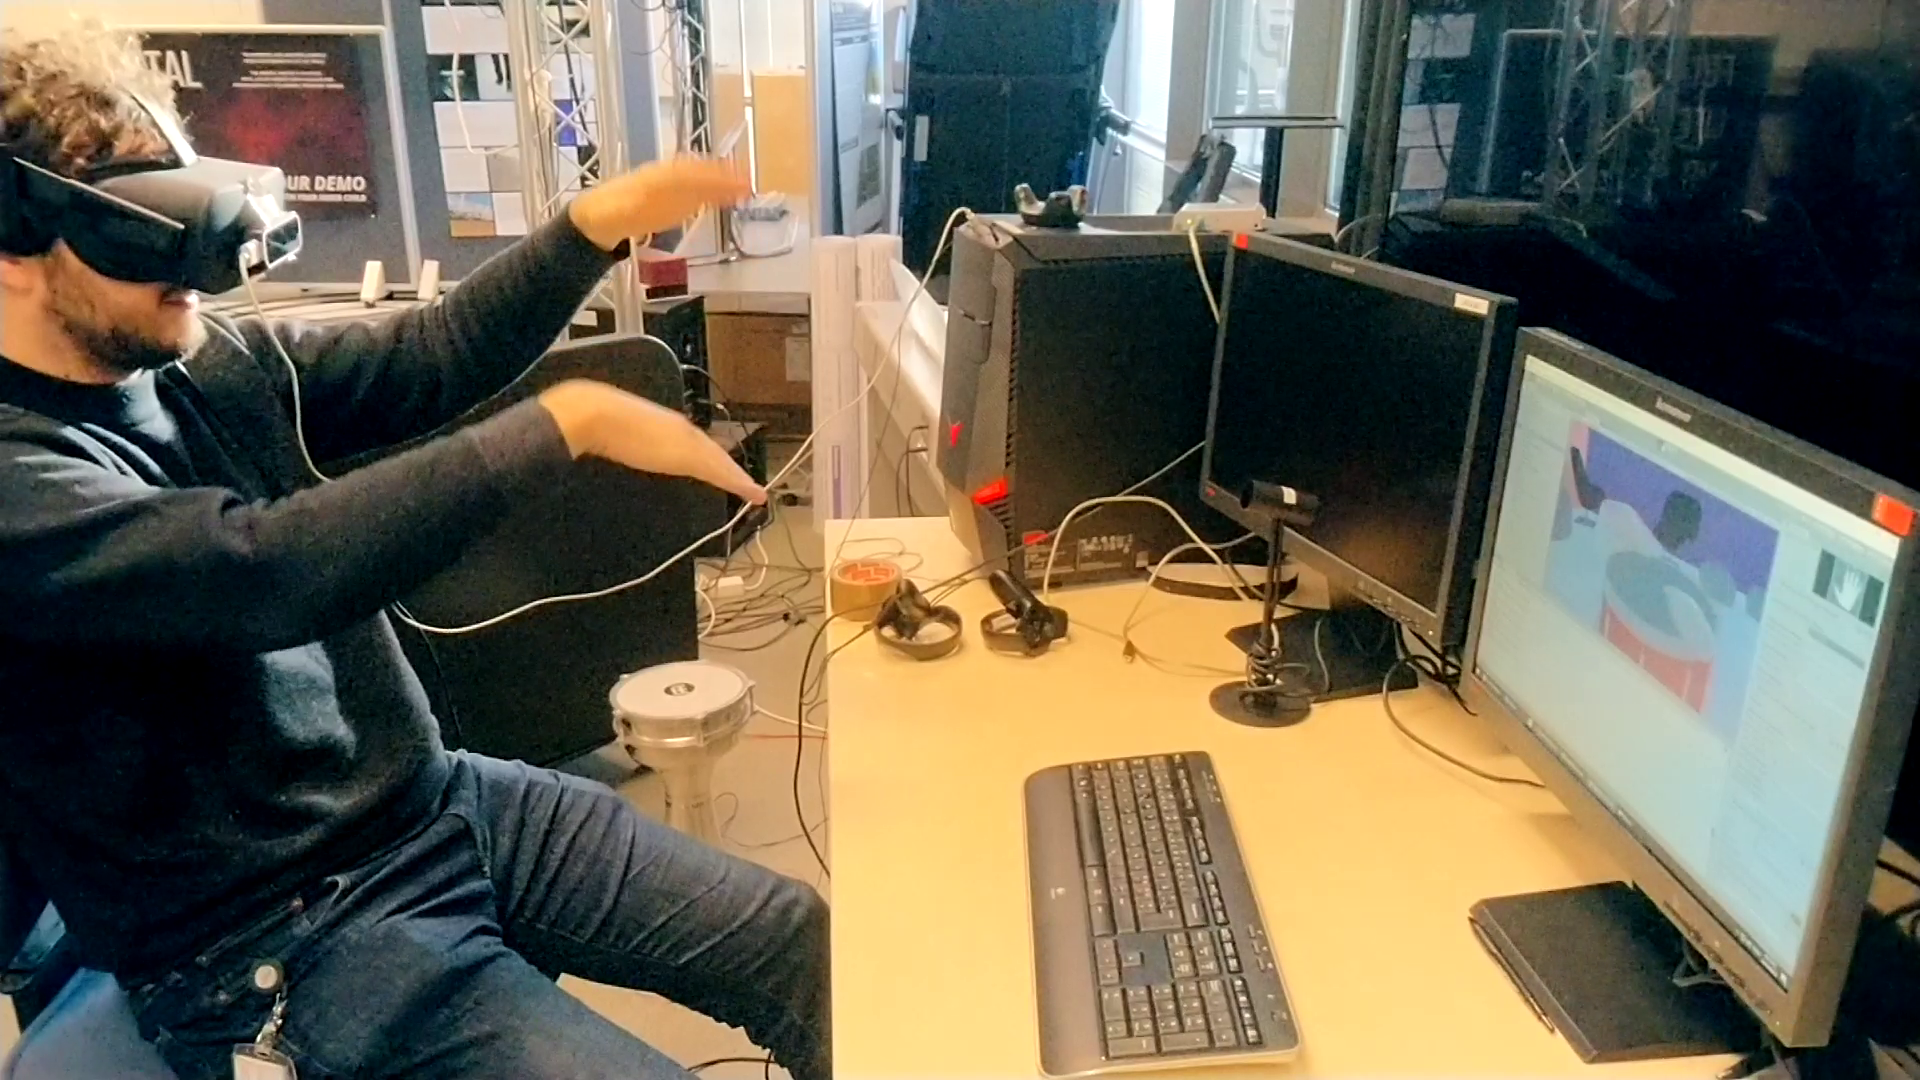
\includegraphics[width=0.5\textwidth]{sil_drum}
%\caption{Leap motion and virtual drum}
%\centering
%\label{fig:sl1}
%\end{figure}
\begin{figure}[h]
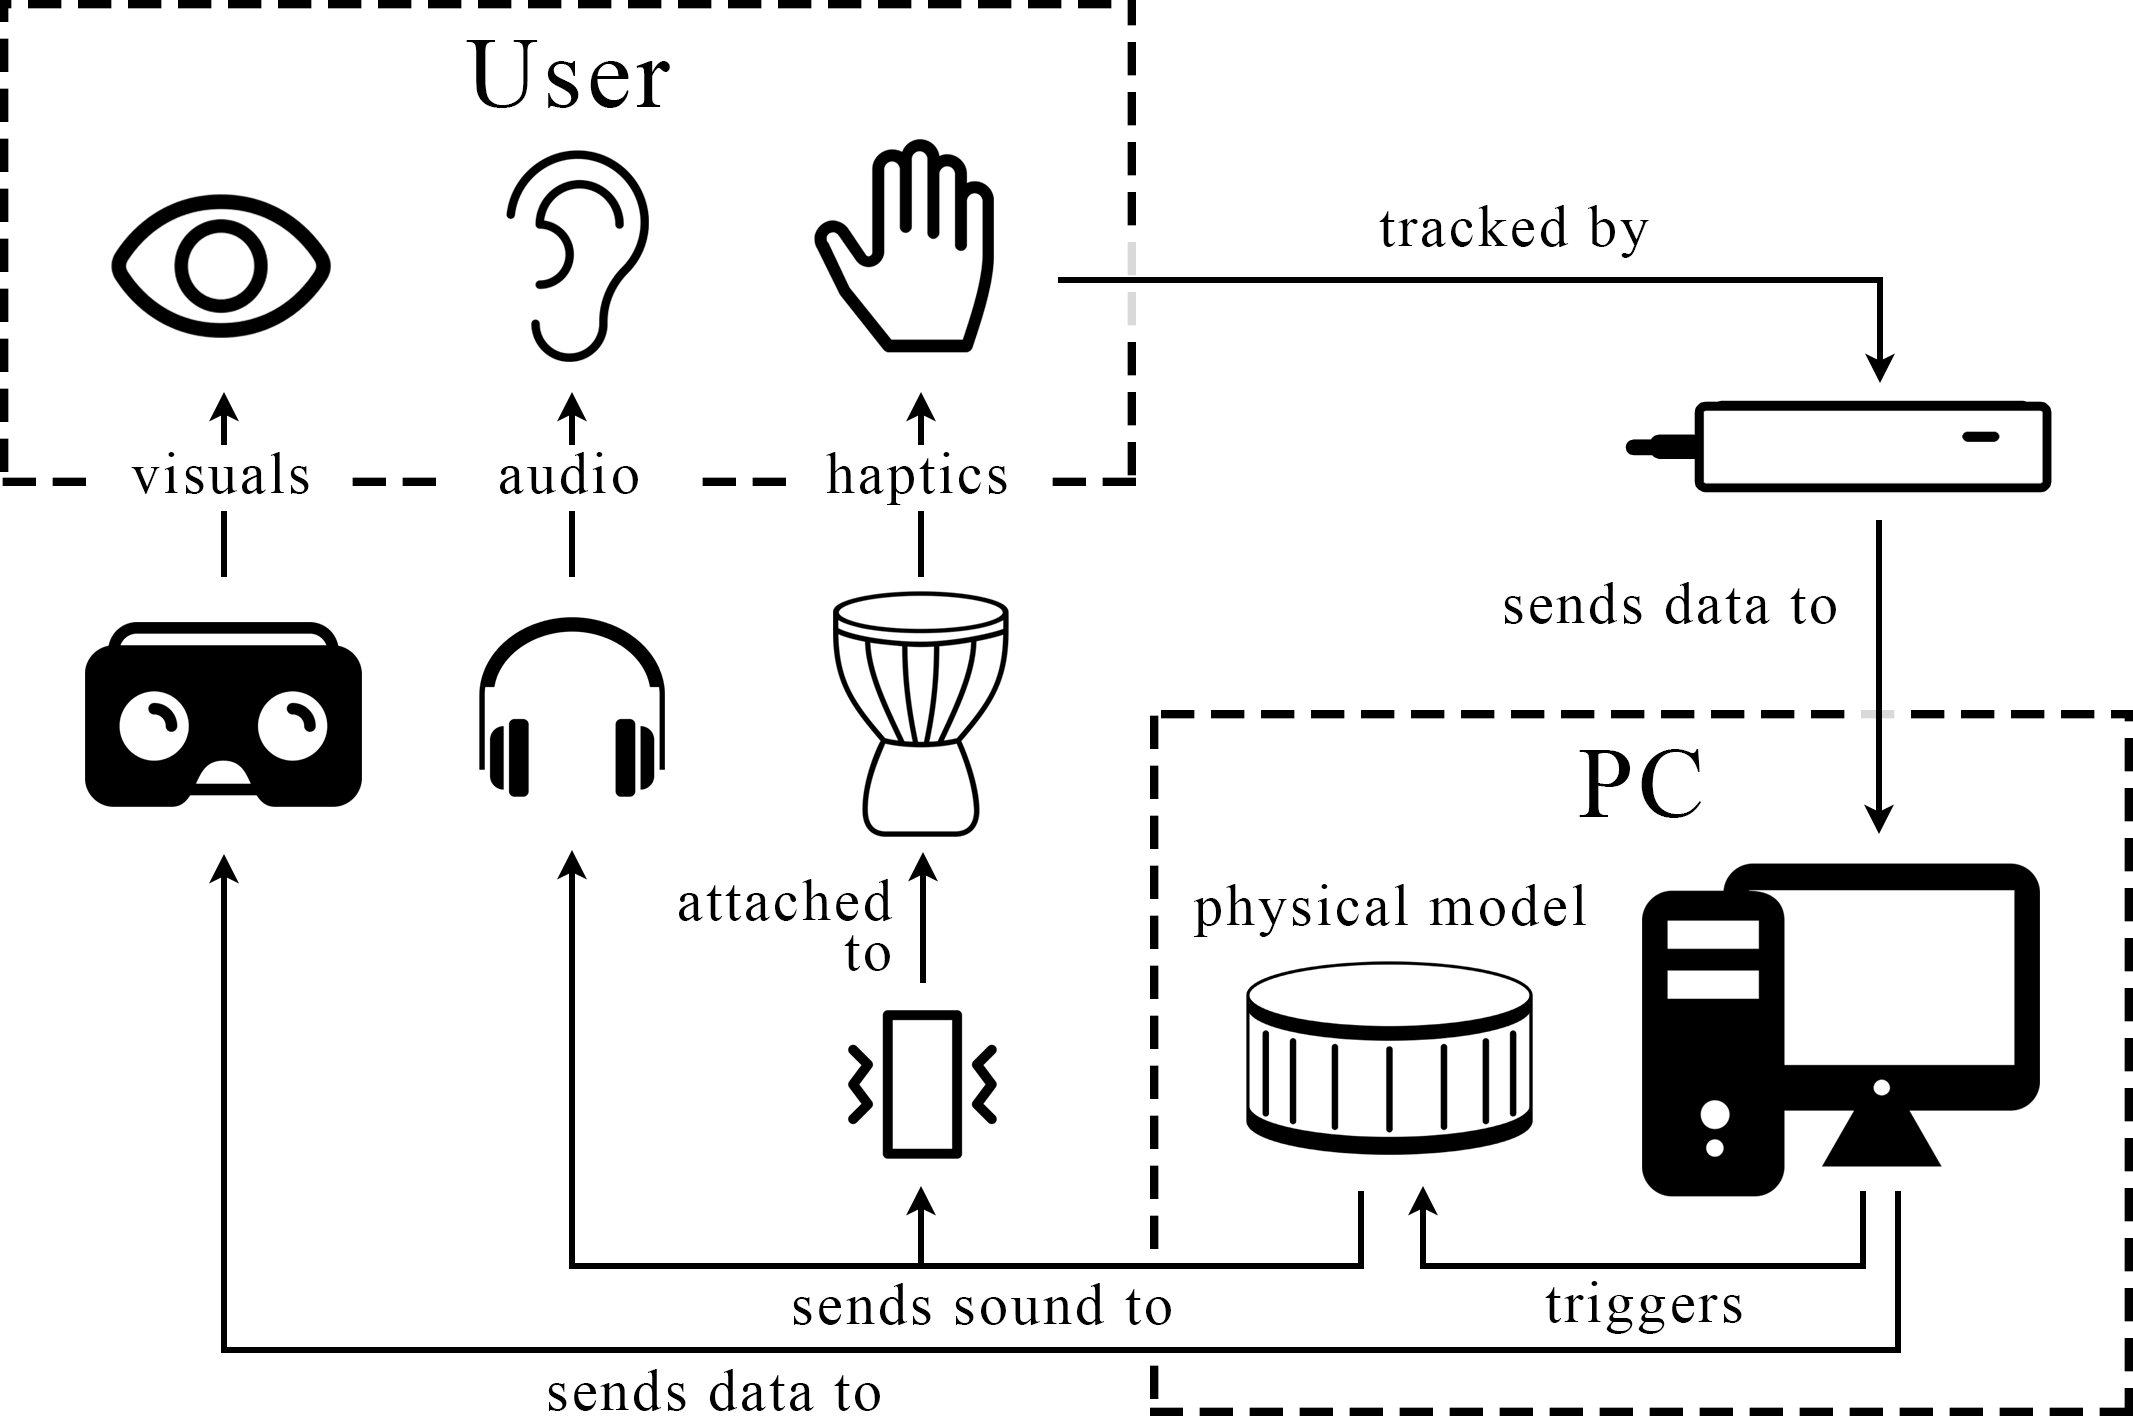
\includegraphics[width=1.0\columnwidth]{systemlayout-updated.png}
\caption{System layout. The user interacts with the system using their hands and gets haptic feedback from the haptuator attached to the drum membrane, auditory feedback from closed headphones and visual feedback from the Oculus Rift headset. A detailed explanation can be found in \autoref{sec:sys}.}
\centering
\label{fig:systemLayout}
\end{figure}

\begin{figure}[h]
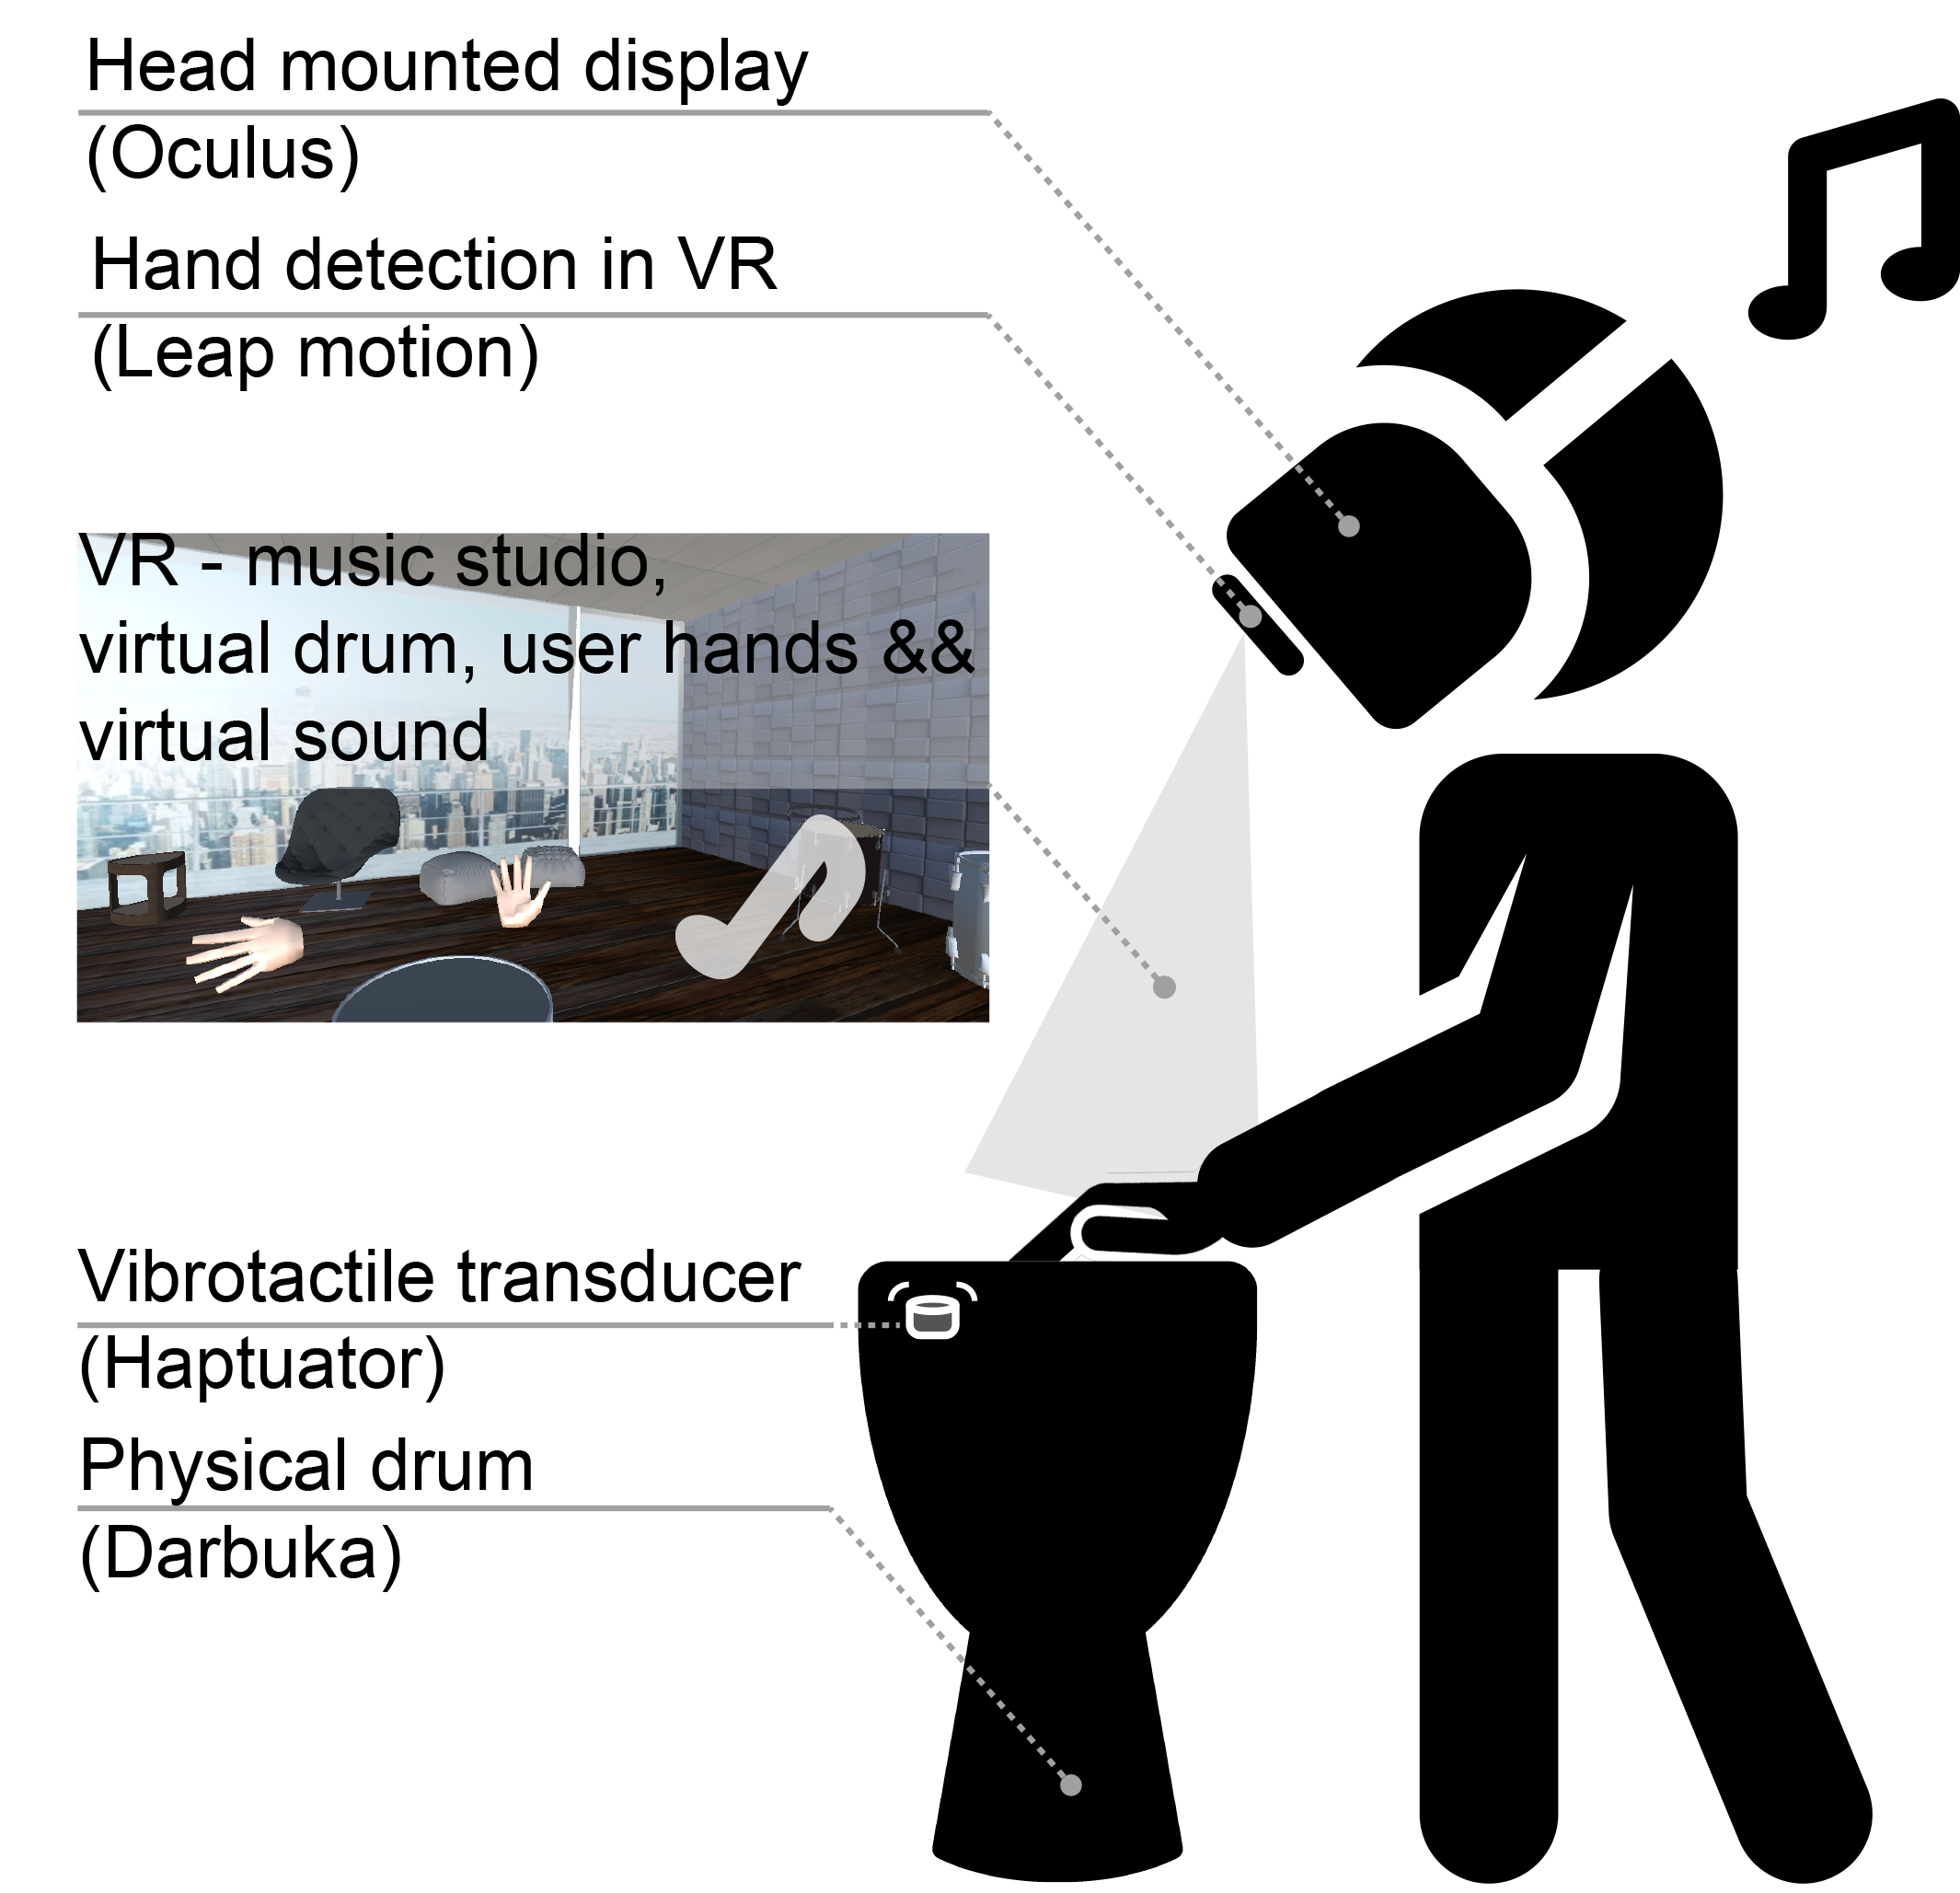
\includegraphics[width=1.0\columnwidth]{VRDrumSetup.png}
\caption{DESCRIPTION HERE. (also, did you code a lot? There's two \&-signs in the description of the visuals ;) )}
\centering
\label{fig:userOverview}
\end{figure}

% \begin{figure}[h]
% \centering
% 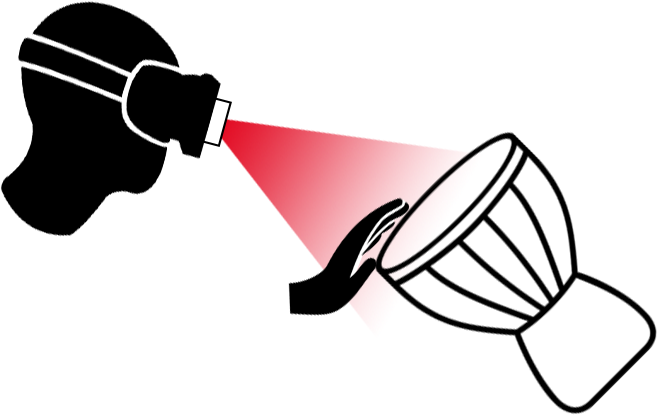
\includegraphics[width=0.7\columnwidth]{leapOnFace.png}
% \caption{The physical setup showing user interaction and tracking. The Leap Motion is mounted on the HMD as shown and tracks the interaction of the hands with the drum.}
% \centering
% \label{fig:userInt}
% \end{figure}

\section{Unity Implementation}\label{sec:unity}
In Unity we created a virtual drum playable with hand motion using the Leap Motion. The user enters the VR environment (rendered as a recording studio) and the Leap Motion reconstructs in VR subject's own hands. In the virtual recording studio we placed a drum at the center of it. Drum skin was programmed to detect collision with the reconstructed hands (each hand had a capsule collider attached to it). When the collision was detected, the C\# script was activated to reproduce the beating sound of the drum through an actuator placed inside the drum skin.

\section{Physical Model}\label{sec:PM}
The behaviour of musical instruments can be well described by partial differential equations (PDEs) \cite{Fletcher1998}. In this section, the continuous-time PDE for a drum-membrane will be given and explained. This is followed by an explanation of the discretisation method after which and parameter values for our implementation will be given. 

\subsection{Continuous time}
A rectangular (stiff) membrane with dimensions $L_x$ (m) and $L_y$ (m) can be described by the following equation \cite{bilbao2009numerical}:

\begin{equation}
\rho H\frac{\partial^2u}{\partial t^2} = T\Delta u - D\Delta\Delta u - 2 \sigma_0\frac{\partial u}{\partial t} + 2 \sigma_1 \Delta \frac{\partial u}{\partial t}.
\end{equation}
Here, state variable, $u = u(x,y,t)$ is a function of horizontal coordinate $x \in [0, L_x]$, vertical coordinate $y \in [0, L_y]$ and time $t\geq0$ and is parameterised in terms of material density $\rho$ (kg/m$^3$), membrane thickness $H$ (m), tension $T$ (N) and frequency independent and dependent damping coefficients $\sigma_0$ (s$^{-1}$) and $\sigma_1$ (m$^2$/s). Furthermore, $D = EH^3/12(1-\nu^2)$ with Young's modulus $E$ (Pa) and Poisson's ratio $\nu$. Lastly, $\Delta$ represents the 2D Laplacian \cite{bilbao2009numerical}:
\begin{equation}\label{eq:PDE}
    \Delta = \frac{\partial^2}{\partial x^2} + \frac{\partial^2}{\partial y^2}.
\end{equation}
Furthermore, clamped boundary conditions -- i.e., the state $u$ at all plate edges and their gradients are 0 -- have been chosen for simplicity:
\begin{equation}
    u = \nabla u = 0 \quad \text{with} \quad \nabla = \frac{\partial}{\partial x} + \frac{\partial}{\partial y}.
\end{equation}
\subsection{Discretisation}
For implementation of the physical model, finite-difference time-domain (FDTD) methods have been used for their accuracy \textbf{SOURCE}. This technique discretises $u(x,y,t)$ shown in Equation \eqref{eq:PDE} to $u_{(l,m)}^n$ using $x=lh$ where $l \in [0, ..., N_x-1]$ and $y=mh$ where $m \in [0, ..., N_y-1]$ where $N_x$ and $N_y$ are the number of horizontal and vertical grid points respectively. Furthermore, time is discretised using $t = nk$ with sample $n$ and time step $k$ (s) and $h$ (m) is the space between two grid points can be calculated using \textbf{source} 
\begin{equation}\label{eq:h}
    h \geq h_\text{min} =  2\sqrt{\frac{c^2k^2 + 4\sigma_1k + \sqrt{(c^2k^2 + 4\sigma_1k)^2 + 4\kappa^2 k^2} }{2}},
\end{equation}
where $c = \sqrt{T/\rho H}$ and $\kappa = \sqrt{D/\rho H}$. The closer $h$ is to $h_\text{min}$, the higher the accuracy of the implementation.
\subsection{Parameters}
Most parameters used in the simulation were chosen using trial and error and empirical tests. They can be found in \autoref{tab:parameters}. With these parameters we will have a small (30$\times$30 cm) membrane with a low density and stiffness. For speed purposes the grid spacing $h$ in Equation \eqref{eq:h} is multiplied by 4. The values for $T$ and $\sigma_0$ correspond to the three different sizes of drum from large to small. Note that we are not changing the size of the model as tension gives the same effect, i.e., changes in frequency. The frequency dependent damping  $\sigma_1$ follows an exponentially decaying curve, 
\begin{equation}
    \sigma_1(t) = 0.005e^{-0.01 t},
\end{equation}
where $t=0$ at the time of excitation. This allows for very low damping, i.e., very long sound, while taking away some of the high frequency content present immediately after excitation.
\begin{table}[h]
\caption{Table showing parameter values}\label{tab:parameters}
\centering
\begin{tabular}{|c|c|c|}
    \hline
    Parameter & Symbol (unit) & Value \\
    \hline
    Membrane width & $L_x$ (m) & $0.3$\\
    Membrane length & $L_y$ (m) & $0.3$ \\
    Material density & $\rho$ (kg/m$^3$)& $10$ \\
    Thickness & $H$ (m) & $0.001$ \\
    Tension & $T$ (N) & $T = \{15, 40, 80\}$ \\
    Young's modulus & $E$ (Pa)& $2\cdot 10^3$ \\
    Poisson's ratio & $\nu$ (-)& $0.3$ \\
    Freq. indep. damping & $\sigma_0$ (s$^{-1}$) & $\sigma_0 \in \{0.5, 2, 5\}$\\
    Freq. dep. damping & $\sigma_1$ (m$^2$/s) & $\sigma_1 \in [0, 0.005]$\\
    Time step & $k$ (s) & $1/44100$\\
    Grid spacing & $h$ (m) & $4h_\text{min}$\\
    \hline
\end{tabular}
\end{table}

\section{Experiment}\label{sec:exp}
%In the above we presented a drum augmented using virtual reality and a vibration motor. Considering that different physical drums would produce different acoustic results and a musician would have to spend hours practicing and improving their stroke techniques for a specific one - our virtual reality musical instrument is an implementation of 3 different drum types into a single setup. While getting the haptic feedback of a drumming experience, one can switch between different musical instruments, explore their potential and train their stroke. 
During the course of this study, we conducted an experiment to reach two goals. Firstly, in order to test how the tension and frequency independent damping coefficient ($T$ and $\sigma_0$ respectively in \autoref{sec:PM}) influence the perception of material stiffness, we inquired this during the experiment.
%How does the perception of material stiffness of a physical drum change when auditory and haptic cues are manipulated in a VR setup?
%How does user interaction with a physical drum change when visual, audio and haptic cues are manipulated in a VR setup?
Secondly, we hoped that the experiment would help us to understand our VRMI's limitations and to inform future development of our work. %Next to finding ways to improve the DigiDrum setup in terms of usability and functionality, 
Furthermore, we hope -- on a larger scale -- to add to the corpus of design guidelines for VRMIs, more specifically those VRMIs which involve a stroking movement. Serafin et al. \cite{Serafin:2016} describe three layers of evaluation for VRMIs, namely: (1) investigating modalities of interaction, (2) evaluating VR specific aspects, with engagement being the most interesting from a VRMI perspective, and (3) looking at quality and goals of interaction. \textbf{\textleftarrow We're not really linking this to anything are we?}

Participants experiences are evaluated through (1) asking them during the test how they rate the stiffness of the material in each of the 9 cases, (2) a questionnaire including questions about their relationship and experience with playing a musical instrument, virtual body ownership and whether they thought interaction patterns changed between the different cases and (3) observation while the participants were interacting with the setup to retrieve data on engagement and stroke patterns which possibly correlate to the haptics and sound.

\subsection{Experiment process}
Before the experiment, participants were told that they would be ``drumming in VR" and that we would test their perception of the stiffness of the material they are interacting with. They were told that they were going to hear 9 different cases in between which the ``parameters of the experience" would be changed and that for each of these cases they would have to rate the stiffness of the material they were interacting with on a scale of 1 to 7, 1 being ``extremely soft or loose", 7 being ``extremely stiff or hard". In between cases, the participant would not take off the headset or headphones. After the test, the participants would fill in a questionnaire with the following questions (the latter two taken from \cite{avanzini2006}):

\begin{itemize}
    \item I felt like the hands in the simulation were my own (1-7 rating)
    \item In order to express your judgements to the questions during the simulation, you relied mainly on... \cite{avanzini2006} (multiple answers possible: visuals\textbar audio\textbar haptics)
    \item In your opinion what was varying between each condition? \cite{avanzini2006} (multiple answers possible: visuals\textbar audio\textbar haptics)
\end{itemize}
From participant observation during the experiment and the the final two questions of the questionnaire, ``Did your behaviour change between different cases, and if so what did you do differently?" and ``Anything you would like to add?", we hoped to get some information on the user interaction and the quality of our setup.

The experiment was done on 16 participants, of which 9 were experienced musicians ($>$ 5 years of instrument practice). Three participants were drummers. 

\section{Results and Discussion}\label{sec:resDisc}
This section will give the results of the experiment and discuss these.
\subsection{Statistical analysis}
The results of the stiffness ratings can be found in \autoref{fig:results}. Intriguingly, we obtained a significant correlation between the stiffness scale and the subjective ratings ($\rho$ = 0.9372, p \textless 0.01) using Spearman correlation. We used the Spearman methodology because number of values is low and we couldn't model a normal distribution \cite{Kirk2007}. As mentioned before, subjective scores ranged from 1 to 7 while we organised the drum stiffness values in 9 levels as shown in Fig. 7.   
\begin{figure}[h]
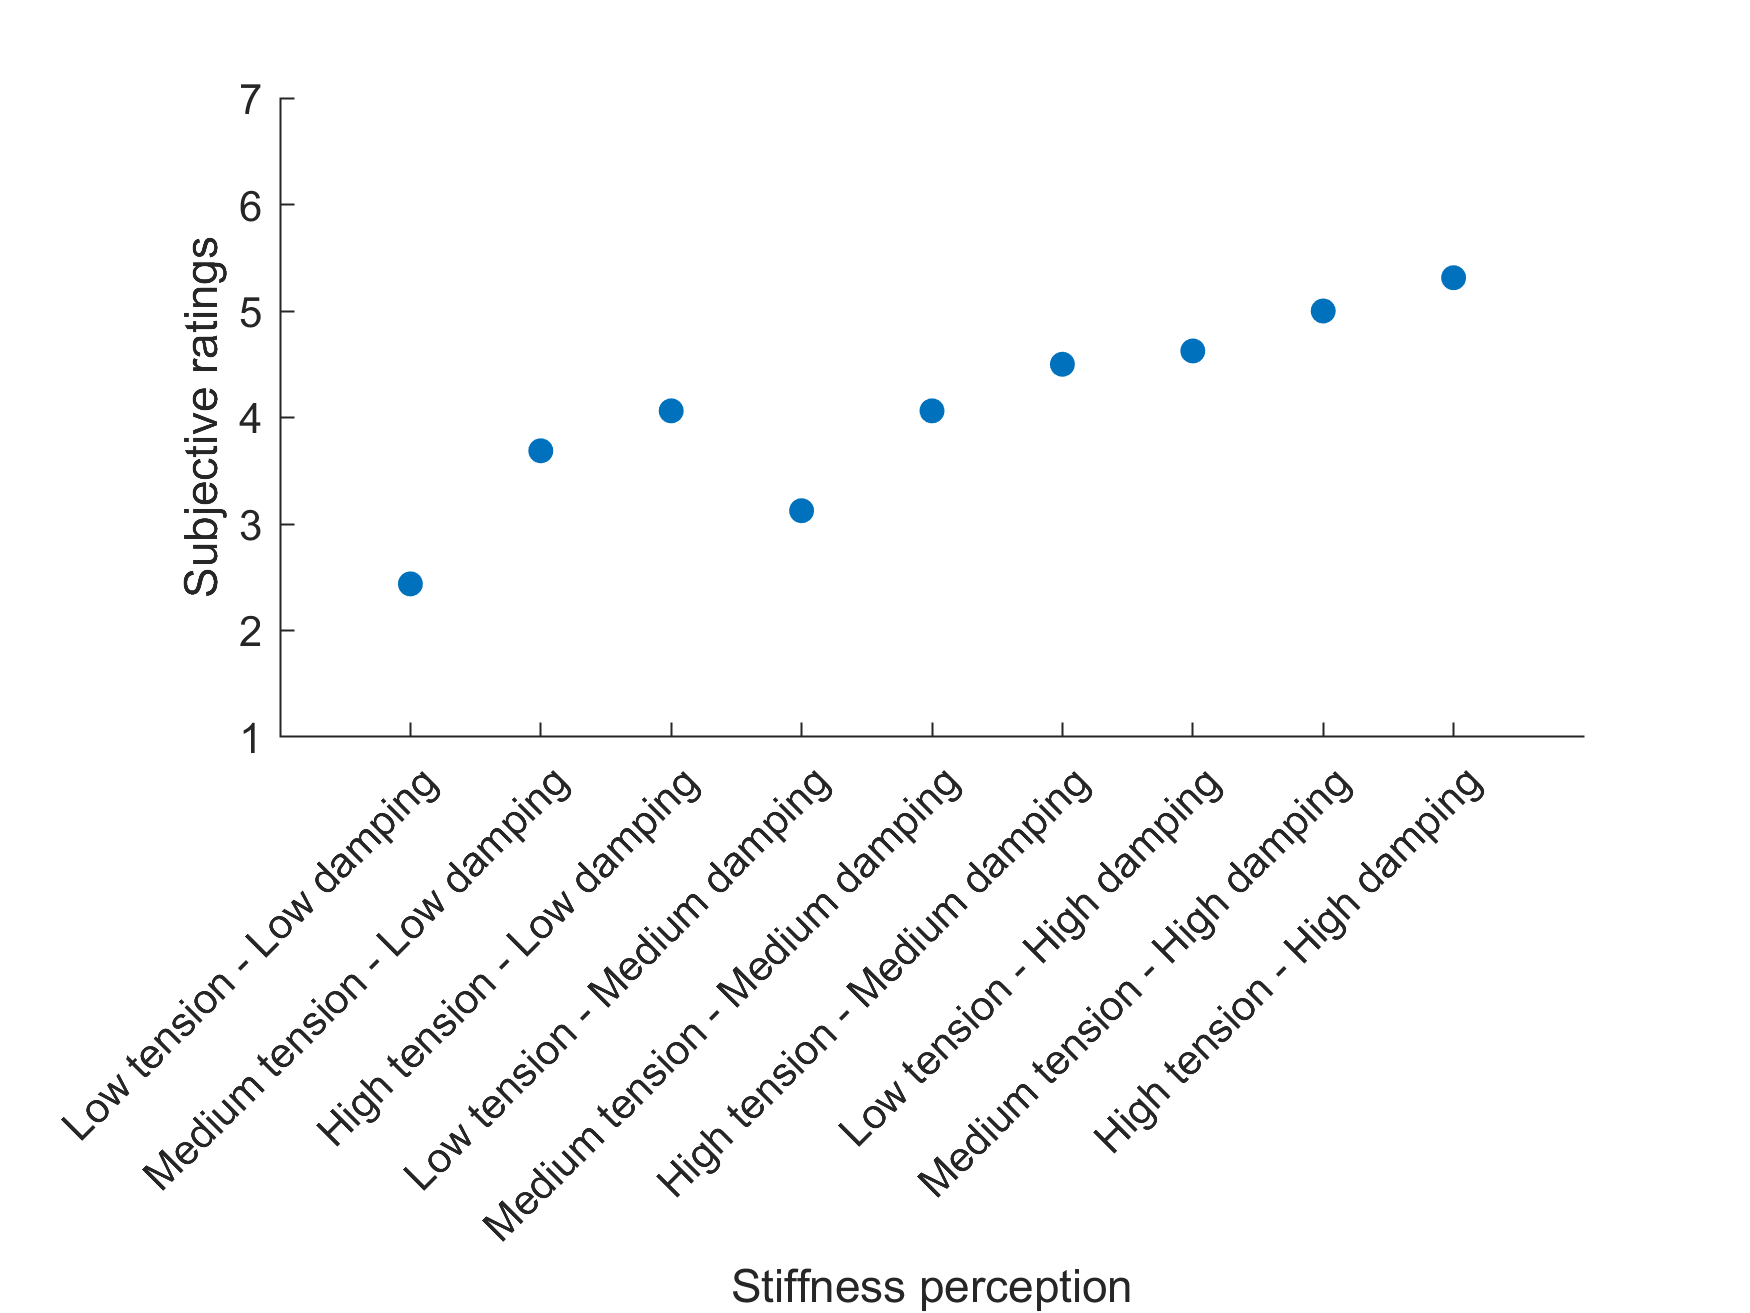
\includegraphics[width=0.5\textwidth]{corr_anal}
\caption{Non-parametric correlation between stiffness and subjective scores}
\centering
\label{fig:results}
\end{figure} 
We can observe a quasi-linear relationship between subjective haptic sensation and the values for tension and samping elicited by the actuator on the drum skin. %It should be noted how lower values of stiffness (between 2 to 4) deviate from the linear trend: subjects had more uncertainty when they had to evaluate lower levels of membrane stiffness. \textbf{this was still assuming that the 9 cases were sorted by stiffness}

\autoref{fig:averagedResults} shows the average participant scores for each level of damping and tension. These two parameters were grouped in levels (low, medium and high) and subjective ranking are plotted as colored bars
\begin{figure}[h]
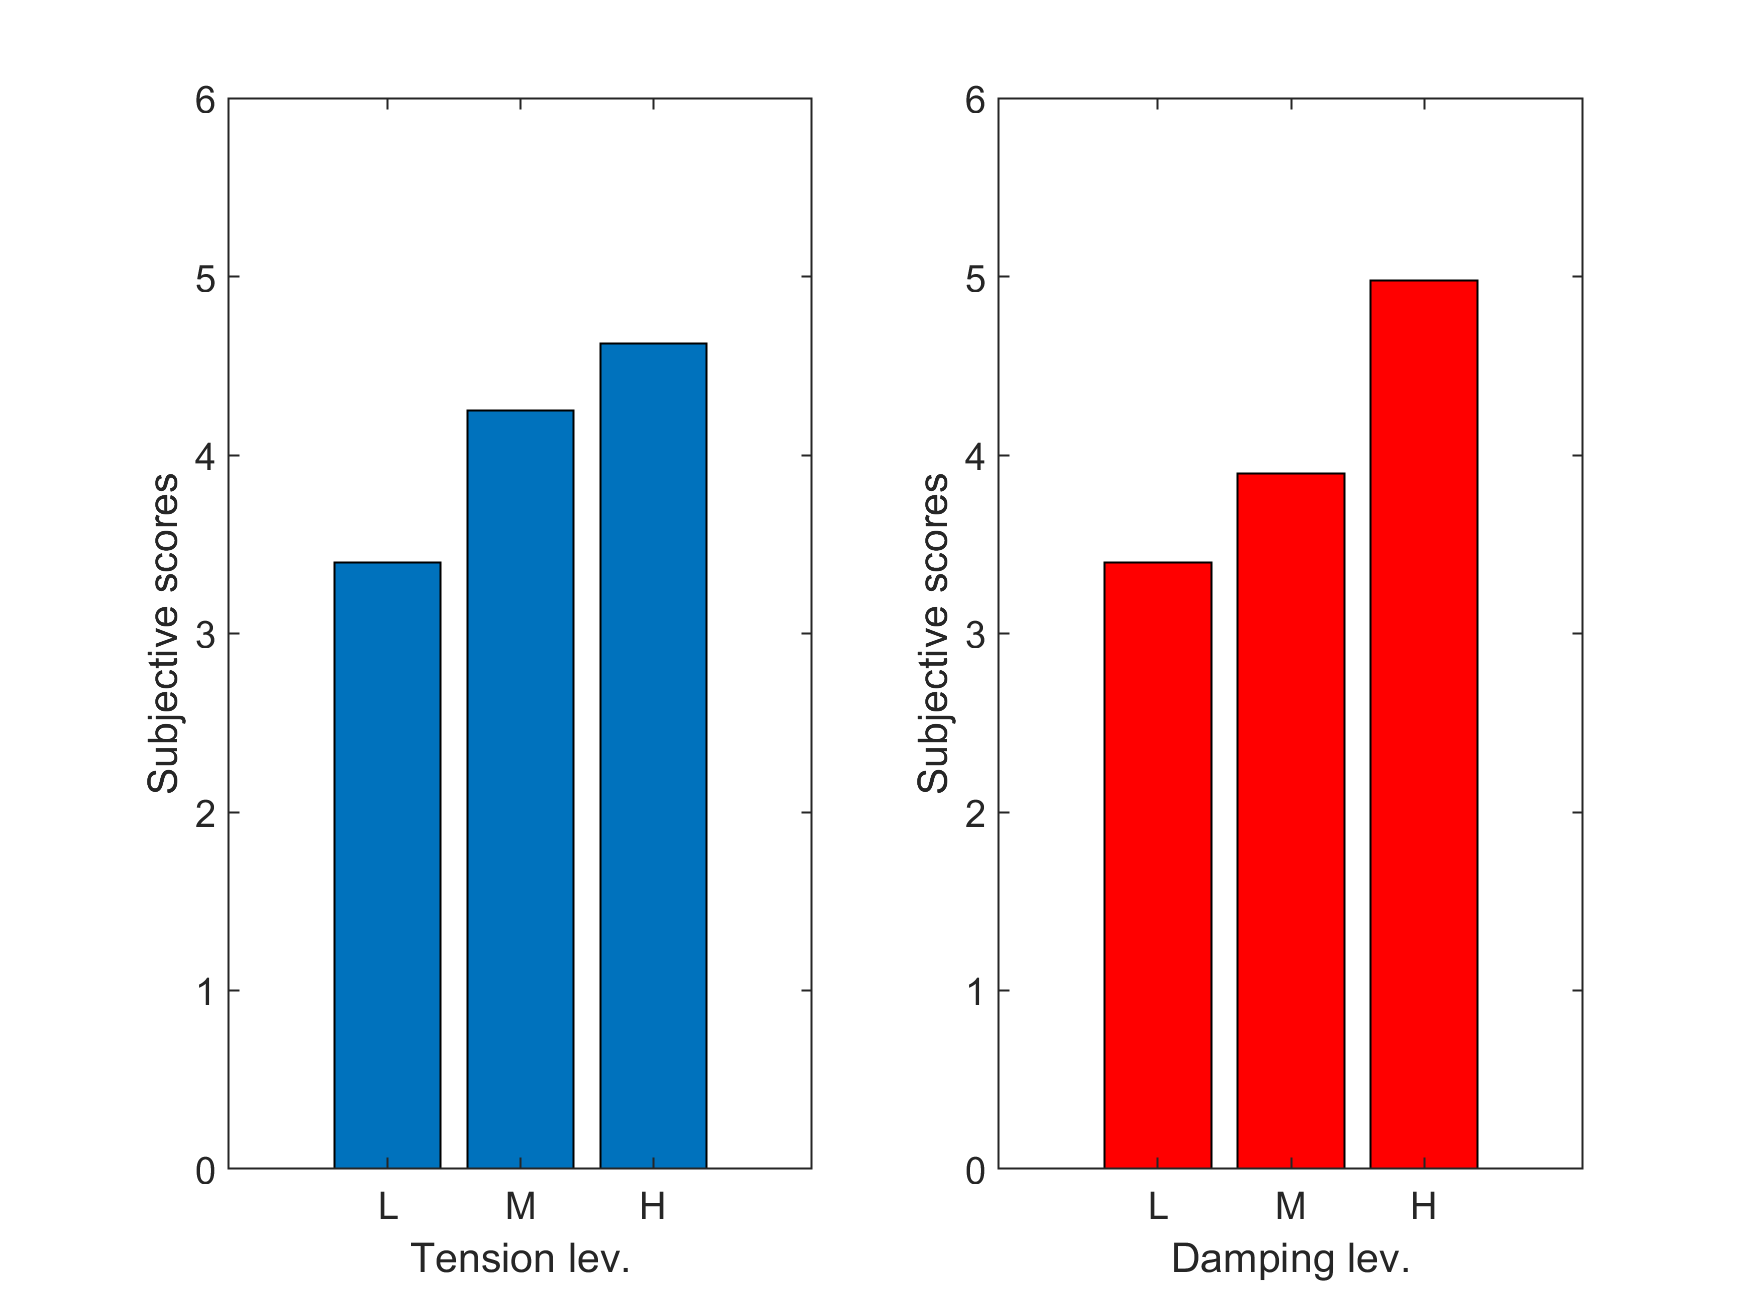
\includegraphics[width=0.5\textwidth]{tens_dump}
\caption{Non-parametric correlation between stiffness and subjective scores}
\centering
\label{fig:averagedResults}
\end{figure} 
We also ran a group level statistical analysis using the Mann-Whitney U-test between tension and damping levels.

We also ran a statistical analysis on each single level based on non-parametric Mann-Whitney U-test and report the results in \autoref{tab:utest}. Abbreviations are T for "tension" and D for "damping" while letters L,M,H mean the level "low","medium" and "high". It is important to take into account the multi-comparison problem and in this case the threshold level for significance should be equal to 0.0056 following the Bonferroni correction.

\def \columnW {0.4cm}
\begin{table}[h!]
\small
\caption{Mann-Whitney U-test (p-values)}
\begin{tabular}{ |p{\columnW}||p{\columnW}|p{\columnW}|p{\columnW}|p{\columnW}|p{\columnW}|p{\columnW}|p{\columnW}|p{\columnW}|p{\columnW}|  }
 \hline
 \multicolumn{10}{|c|}{Mann-Whitney U-test [p values]} \\
 \hline
  & LT LD & MT LD & HT LD & LT MD & MT MD & HT MD & LT HD & MT HD & HT HD \\
 \hline
LT LD &	 &	.0642 &	.0163 &	.1268 &	.0049 &	.0041 &	.0034 &	.0004 &	.0002\\
\hline
MT LD &	.0642 &	 &	.6463 &	.3465 &	.6582 &	.1802 &	.1584 & 	.034 &	.0091\\
\hline
HT LD &	.0163 &	.6463 &	 &	.2123 &	.8933 &	.5413 &	.4455 &	.1737 &	.0915\\
\hline
LT MD &	.1268 &	.3465 &	.2123 &	 &	.0791 &	.0254 &	.0283 &	.0012 &	.0009\\
\hline
MT MD &	.0049 &	.6582 &	.8933 &	.0791 &	 &	.3191 &	.3114 &	.0449 &	.0174\\
\hline
HT MD &	.0041 &	.1802 &	.5413 &.0254 &	.3191 &	 &	.7732 &	.5214 &	.1383\\
\hline
LT HD &	.0034 &	.1584 &	.4455 &	.0283 &	.3114 &	.7732 &	 &	.7725 &	.3424\\
\hline
MT HD &.0004 &	.034 &	.1737 &	.0012 &	.0449 &	.5214 &	.7725 &	 &	.2991\\
\hline
HT HD &	.0002 &	.0091 &	.0915 &	.0009 &	.0174 &	.1383 &	.3424 &	.2991 &	\\

 \hline
 \multicolumn{10}{|c|}{Note: Bonferroni adjusted significance threshold for multi-comparison p\textless0.0056} \\
 \hline
\end{tabular}
\label{tab:utest}
\end{table}

As we can observe from \autoref{tab:utest}, there isn't a significant difference between "high tension - low damping" and "low tension - medium damping" (p=0.2123) suggesting that the linear relation of Figure 7 holds despite the "step" or the discontinuity between points as seen on the scatterplot. However, we should consider it similar to a monotonically increasing function rather than a pure linear trend. 

Lastly, \autoref{tab:groupComp} shows group comparisons between the three different values of damping and tension. 
\begin{table}[t]
\centering
\caption{Comparison between different levels of Tension and Damping}\label{tab:groupComp}
\begin{tabular}{ |c|c|c| } 
 \hline
 \multicolumn{2}{| c |}{Different levels of tension/damping} & p-values\\
 \hline
 Low Damping & Medium Damping & 0.2560 \\ 
 Medium Damping & High Damping & 0.0078 \\
 Low Damping & High Damping & 6.5071e-04 \\
 Low Tension & Medium Tension & 0.0950 \\
 Medium Tension & High Tension & 0.4268 \\
 Low Tension & High Tension & 0.0297 \\
 \hline
\end{tabular}
\end{table}
From Table 3 outcomes, we can notice a significant difference in participant's ratings between  medium-high damping and low-high damping levels while tension shows significance only between low to high tension. We could hypothesize that damping is a factor that drives participants' tactile experience more than tension. Another observation is that it appears difficult for participants to evaluate low to medium levels of both damping and tension. 
\subsection{Statistical analysis: reliability}
Indivual ratings were initially analyzed with Cronbach's alpha \cite{Cronbach1951} to test the internal consistency of the responses. This measure is generally known as a metric of reliability with higher values of alpha as those  more desirable. The unstandardized Cronbach's alpha value was 0.6348 while the standardized value reached 0.6589. According to \cite{Kline2000}, a value between 0.6 to 0.7 is questionable with 0.7 as the threshold for an acceptable test. Despite the consistency outcomes, it appears that in future we could easily reach the reliability threshold just increasing the sample size. Moreover, if we don't consider all factors loadings as evenly distributed, we could assume that the Cronbach's alpha underestimates the true reliability. 

\subsection{Questionnaire}
As can be seen from the questionnaire results in \autoref{tab:results} the participants generally found that the hands in the simulation were their own. This proves that the Leap Motion is a good way to track the hands and that this was well implemented. Moreover, it is clear that the visuals had no influence on participants' judgement, most probably because they were unchanged. The audio, however, seemed to be the most predominant feature that the users focused on when expressing their judgements (93.8\%). Haptics for expressing judgements was only chosen by 5 participants (31.3\%). In the future, removing the audio, only leaving the haptics might be a better way to force the user to use their sense of touch and test its influence on perception.

\begin{table}[t]
\caption{Questionnaire results. The last two questions were taken from \cite{avanzini2006}.}\label{tab:results}
\centering
\begin{tabular}{|p{6cm}|p{1.5cm}|}
    \hline
    Question & Result \\
    \hline
    \vspace{0.05em}
    I felt like the hands in the simulation were my & \vspace{0.05em}$\mu = 5.44$,\\
    own. (1-7 rating) & $\sigma = 1.26$ \\
    & \\
    In order to express your judgements to the ques- & visuals: \, 0,\\
    tions during the simulation, you relied mainly & audio: \: 15, \\ on... (visuals\textbar audio\textbar haptics) & haptics: \: 5 \\
    &\\
    In your opinion what was varying between each & visuals: \, 0, \\
    condition? (visuals\textbar audio\textbar haptics) & audio: \: 14,\\
    & haptics: 10 \\
    \hline
\end{tabular}
\end{table}

\subsection{Other observations}
From participant observation during the experiment, comments they gave during and after the test, and the two last (open) questions of the questionnaire (see \autoref{sec:exp}) we obtained some extra findings. 

Due to the fact that the virtual drum was placed slightly higher than the physical drum (see \autoref{sec:sys}), many participants interacted with the air above the drum rather than finishing their stroke to actually hit the drum. This was an issue, as the haptic sensation would not be felt in that case. Either before or during the test, the participants were instructed to finish their stroke to actually physically interact with the drum. 
Furthermore, the interaction was programmed in such a way, that when a tracked hand collides with the virtual drum, this hand would not be able to trigger the physical model until it was completely out of the ``collision zone". Due to the misalignment mentioned above, many interactions were not captured. Again, either before or during the experiment, the participants were instructed to make longer movements to ensure that their hands were completely outside of this ``collision zone" before interacting with the drum again.

Another technical issue was that sometimes participants would look forward rather than down to the hands which caused the hands not to be tracked anymore. A solution for this would be to mount the Leap Motion in a way that it tracks more down rather than straight forward (as is the case now).

Some participants commented that they would have liked to have reference points for ``the stiffest" and ``the softest" cases as they said they would have judged the first few cases differently if they had known these references in advance.

The movements of participants were observed during the test and sporadically noted. There was a small tendency towards slower and longer movements in the case of lower tension and faster and shorter movements in the opposite case, but as these observations were not done systematically, this should be properly tested using raw data from the hand tracking.

%The physical model of the membrane allows for sound experimentation with sounds which 
%In this paper we presented a setup made of: a virtual reality drum which involves a physical prop providing haptic feedback. Considering that different physical drums would produce different acoustic results and a musician would have to spend hours practicing and improving their stroke techniques for a specific one - our virtual reality musical instrument is an implementation of 3 different drum types into a single setup. While getting the haptic feedback of a drumming experience, one can switch between different musical instruments, explore their potential and train their stroke. This takes advantage of the fact that VR allows for possibilities which could not happen in the real world.

\section{Conclusion}\label{sec:conc}

In this paper we presented and evaluated a novel VRMI where a physical drum was enhanced by virtual reality. The physical drum was augmented by a vibration motor and the sound was simulated using a physical model of a drum membrane.

Future work includes decoupling the audio and the haptics, to test the perceptual influence of each in individual modality separately. Next to that, the tracking of the user's hands should be improved by mounting the Leap Motion more downwards on the HMD. Furthermore, the virtual and physical drum should be better aligned in space as to make the interaction less confusing and more intuitive. Lastly, in order to test whether the interaction patterns change depending on the changes in parameters, the raw data from the hand tracking should be analysed. As an addition to this, the Myo could be used to get more complex interaction data.

%% if specified like this the section will be committed in review mode
\acknowledgments{
The authors wish to thank Stefania Serafin, Cumhur Erkut, Niels Nilsson, Rolf Nordahl, and Michele Geronazzo - our teachers of the ``Virtual, Augmented, Mixed realities" PhD course at Aalborg University Copenhagen for their help during the process of this project.}

%\bibliographystyle{abbrv}
\bibliographystyle{abbrv-doi}
%\bibliographystyle{abbrv-doi-narrow}
%\bibliographystyle{abbrv-doi-hyperref}
%\bibliographystyle{abbrv-doi-hyperref-narrow}

\bibliography{template}
\end{document}
